%
% operation.tex
%
% Copyright The TTC 2.0 Contributors.
%
% TTC 2.0 Documentation
%
% This work is licensed under the Creative Commons Attribution-ShareAlike 4.0
% International License. To view a copy of this license,
% visit http://creativecommons.org/licenses/by-sa/4.0/.
%

%
% \brief Introduction chapter.
%
% \author Gabriel Mariano Marcelino <gabriel.mm8@gmail.com>
%
% \version 0.3.0
%
% \date 2022/10/09
%


\chapter{Operation} \label{ch:operation}

This chapter describes general aspects of the TTC operation, like details of the used communication protocol, how to transmit a packet, how the telecommand reception works, and so on.

\section{Packet transmission}

To transmit a packet, the command ``Transmit Packet'' must be used (\autoref{sec:commands}). When the TTC receives this command through one of its command interfaces, a new NGHam packet is generated with the command content as the packet's payload. After the NGHam packet is generated, it is transmitted immediately through the air using the respective TTC's radio.

\section{Telecommand reception}

When a new valid telecommand is received, it is stored in an internal queue with five positions and 300 bytes available for each position. The new packet is discarded if the queue is full and there are no available positions to store the telecommands.

A telecommand is only stored if it is a valid NGHam packet, and only the payload of the NGHam packet is stored. Each telecommand can be up to 220 bytes long, according to the NGHam protocol definitions.

The received and stored telecommand can be read with the command read packet, as described in \autoref{sec:commands}. After a telecommand is read, it is deleted from the internal queue of the TTC module. The number of available telecommands and the length in bytes of the first queue position can be read using the command ``Read Parameter'', as also described in \autoref{sec:commands} and \ref{sec:variables}.

\section{Communication protocol}

The communication protocol used with the satellite is the NGHam \cite{pyngham-doc}. The NGHam protocol stands for Next Generation Ham Radio, a protocol designed for packet communication. It is similar to the classical AX.25 \cite{ax25} protocol, but with the idea of using a FEC (Forward Error Correction) algorithm to increase the robustness, as defined in \cite{lofaldli2016}:

\begin{quote}
``...a link protocol partly inspired by AX.25. To improve the link reliability, it features Reed Solomon codes for Forward Error Correction (FEC). This makes the data transmission more robust compared to, i.e., AX.25, which does not directly implement FEC on the link layer.''
\end{quote}

It was initially developed in the context of the CubeSat NUTS-1 (NTNU Test Satellite) development by the Norwegian University of Science and Technology (NTNU). This library is based on the implementation of Jon Petter Skagmo (LA3JPA), available in \cite{ngham}.

\subsection{Packet fields}

The \autoref{fig:ngham-pkt} presents a diagram with packet format and the data fields of the NGHam protocol.

\begin{figure}[!ht]
    \begin{center}
        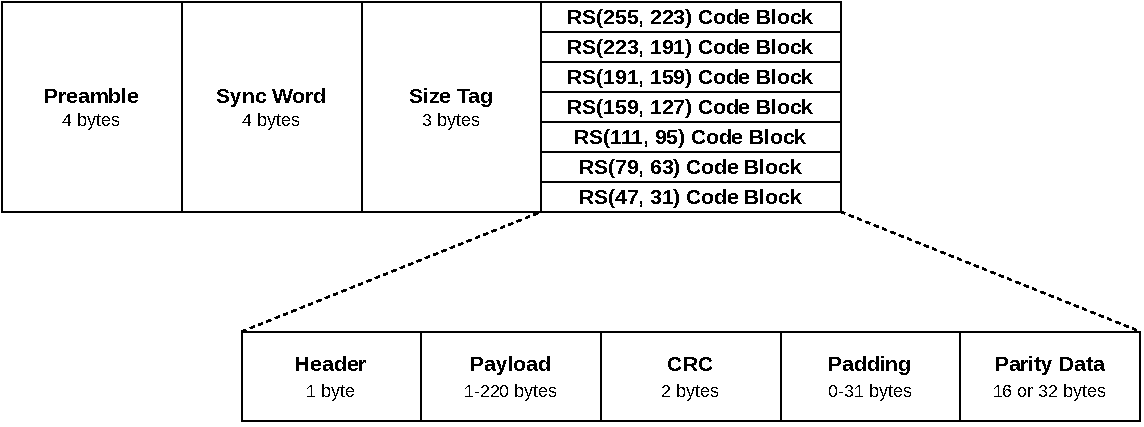
\includegraphics[width=\textwidth]{figures/ngham-pkt.pdf}
        \caption{Format of an NGHam packet.}
        \label{fig:ngham-pkt}
    \end{center}
\end{figure}

Next, there is a brief description of each one of those fields.

\subsubsection{Preamble}

Considering a data rate of 9600 bps, 4 bytes are typically used for the preamble. This sequence is an alternation of ones and zeros: 4$\times$ 0xAA (0b10101010).

\subsubsection{Sync. word}

The sync. word is a sequence of bits used for packet synchronization. With this sequence, the receiver can detect the start of a new packet. In NGHam, the sync. word is composed of 32 bits, following the pattern: 0x5D, 0xE6, 0x2A, 0x7E.

\subsubsection{Size tag}

This field indicates one of the seven possible packet sizes. It is a 24 bits tag and is made very robust by keeping a hamming distance of 13 bits between all vectors. The seven possible tags are listed in \autoref{tab:ngham-sizes}.

\begin{table}[!ht]
    \centering
    \begin{tabular}{llll}
        \toprule[1.5pt]
        \textbf{Size Num.} & \textbf{Tag} & \textbf{Reed-Solomon Config.} & \textbf{Max. Data Size} \\
        \midrule
        1 & 59, 73, 205   & RS(47, 31)   & up to 28 bytes of data \\
        2 & 77, 218, 87   & RS(79, 63)   & up to 60 bytes of data \\
        3 & 118, 147, 154 & RS(111, 95)  & up to 92 bytes of data \\
        4 & 155, 180, 174 & RS(159, 127) & up to 124 bytes of data \\
        5 & 160, 253, 99  & RS(191, 159) & up to 156 bytes of data \\
        6 & 214, 110, 249 & RS(223, 191) & up to 188 bytes of data \\
        7 & 237, 39, 52   & RS(255, 223) & up to 220 bytes of data \\
        \bottomrule[1.5pt]
    \end{tabular}
    \caption{NGHam packets sizes.}
    \label{tab:ngham-sizes}
\end{table}

\subsubsection{Reed-Solomon block}

The Reed-Solomon code block (or just RS block) is the field with packet payload and parity data. It is divided into two parts: data and parity bytes. The data bytes are subdivided into four fields: header, payload, checksum, and padding. Each one of these fields is described below.

\paragraph{Header}

The header byte is the first data byte of the RS block. It is divided as presented in \autoref{tab:ngham-header-flags}.

\begin{table}[!ht]
    \centering
    \begin{tabular}{ll}
        \toprule[1.5pt]
        \textbf{Bits} & \textbf{Purpose} \\
        \midrule
        7 to 6  & Reserved \\
        5       & Extension on \\
        4 to 0  & Padding size (in bytes) \\
        \bottomrule[1.5pt]
    \end{tabular}
    \caption{NGHam header flags.}
    \label{tab:ngham-header-flags}
\end{table}

The extension bit indicates if the extension frame is enabled or not. The padding size bits are the number of padding bytes presented in the respective packet (0 to 31).

\paragraph{Payload}

The payload field is where the “useful” packet data is stored. As presented in the Size Tag field description above, each of the seven size groups allows a maximum number of bytes in the packet payload. The maximum possible length of the payload for an NGHam packet is 220 bytes. If more data need to be transmitted, it should be divided into chunks of 220 bytes and transmitted in separate packets.

\paragraph{Checksum}

There is a checksum field after the payload data to ensure data correctness and a first stage before running the Reed-Solomon correction algorithm. The used checksum algorithm is the CRC16-CCITT 5, with the following configuration:

\begin{itemize}
    \item \textbf{Polynomial}: 0x1021
    \item \textbf{Initial value}: 0xFFFF
    \item \textbf{Final XOR value}: 0xFFFF
\end{itemize}

The CRC16 value is computed from the header and the payload fields.

If the CRC16 value is correct, the Reed-Solomon chain is skipped, and the packet is directly considered valid. This way, the checksum field also allows a performance improvement.

\paragraph{Padding}

To ensure the right packet length for the Reed-Solomon coding in use, if the payload content is less than the maximum allowed, the data field of the RS block is padded with zeros. The number of padding bytes is declared in the header byte (bits 4-0).

\paragraph{Parity data}

This field is reserved for the computed parity bytes of the Reed-Solomon coding algorithm. The used implementation of the RS algorithm is based on the famous FEC library developed by Phil Karn (KA9Q) 6. This field can be 16 or 32 bytes long, depending on the payload length, and consequently, the adopted RS scheme described in \autoref{tab:ngham-parity}.

\begin{table}[!ht]
    \centering
    \begin{tabular}{lll}
        \toprule[1.5pt]
        \textbf{Size Num.} & \textbf{Reed-Solomon Config.} & \textbf{Parity bytes} \\
        \midrule
        1 & RS(47, 31)   & 16 \\
        2 & RS(79, 63)   & 16 \\
        3 & RS(111, 95)  & 16 \\
        4 & RS(159, 127) & 32 \\
        5 & RS(191, 159) & 32 \\
        6 & RS(223, 191) & 32 \\
        7 & RS(255, 233) & 32 \\
        \bottomrule[1.5pt]
    \end{tabular}
    \caption{.}
    \label{tab:ngham-parity}
\end{table}

For the Reed-Solomon framing, the following configuration is used:

\begin{itemize}
    \item \textbf{Symbol size}: 8
    \item \textbf{GF polynomial}: 0x187 (coefficients form)
    \item \textbf{First root of RS code generator polynomial}: 112 (index form)
    \item \textbf{Primitive element}: 11
    \item \textbf{Number of roots}: 16 or 32 (table above)
\end{itemize}

\subsection{Scrambling}

Before transmitting a packet, the RS code block is scrambled by making a byte xor operation with a pre-generated table based on the polynomial $x^{8} + x^{7} + x^{5} + x^{3} + 1$ (defined in the CCSDS 131.0-B-3 standard \cite{ccsds}).

When the receiver receives a packet, it also performs the same operation to de-scramble the RS code block and gets the original content of the RS part of the packet.

By scrambling the packets, long sequences of ones or zeros are avoided by guaranteeing a good bit transition along the whole packet. More information about packet scrambling (or randomization) can be found in \cite{ccsds} (section 8.3).

\section{Flow of execution}
The TTC module operates accordingly to the flowchart from Figure \ref{fig:ttc_flowchart}. Its routine consists of frequent checks for uplink packages or requests from OBDH or EPS to downlink data. Also, by default TTC has protective measures to reset the radio between 600 seconds and the microcontroller after 10 hours.

\begin{figure}[!ht]
    \begin{center}
        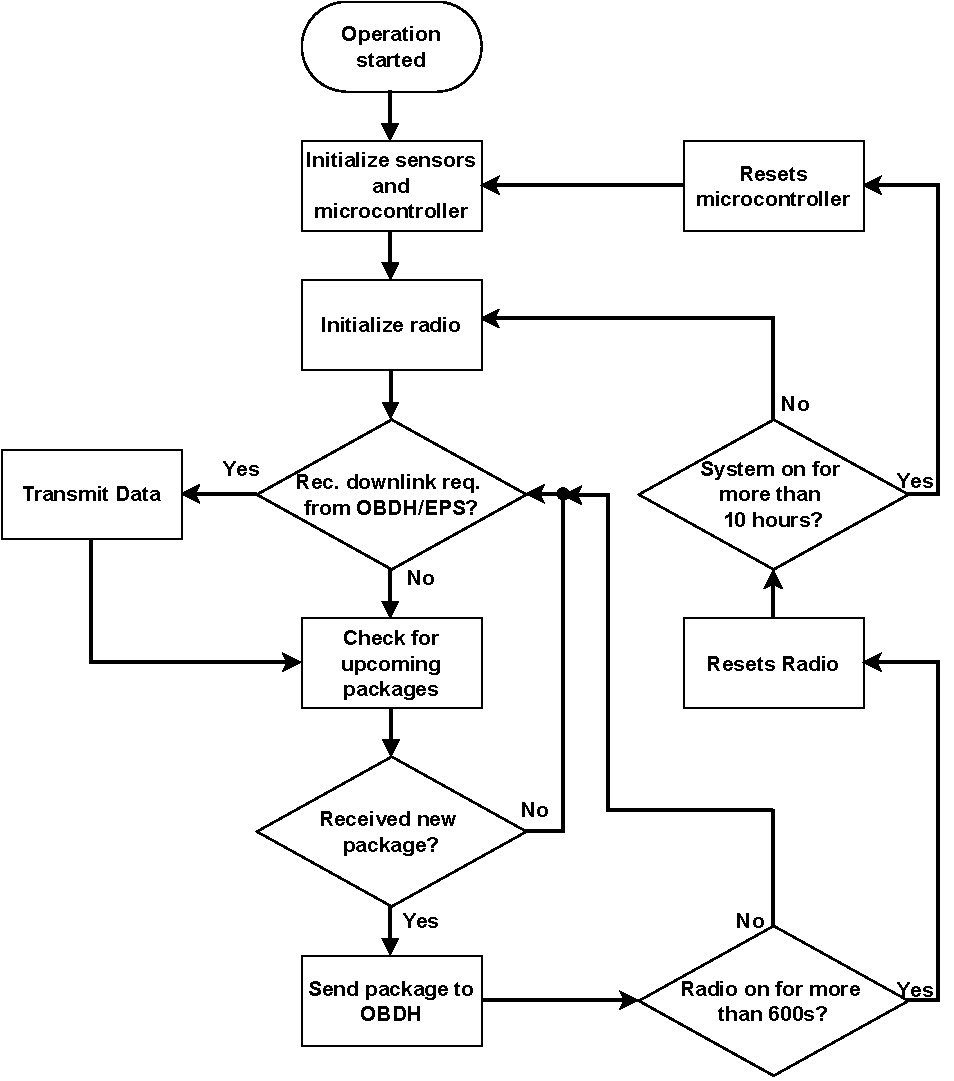
\includegraphics[width=\textwidth]{figures/ttc2-flowchart.pdf}
        \caption{TTC 2.0 flowchart of execution.}
        \label{fig:ttc_flowchart}
    \end{center}
\end{figure}